\chapter{Implementation}

This chapter discusses the technical implementation of the Recruitment Portal, covering the development environment, technology stack, and core logic for file management and security.

\section{Technology Stack}

The system is built using the MERN stack. Table \ref{tab:stack} summarizes the primary technologies used.

\begin{table}[htbp]
  \centering
  \caption{Recruitment Portal Technology Stack.}
  \label{tab:stack}
  \begin{tabularx}{\textwidth}{llX}
    \hline
    \textbf{Component}    & \textbf{Technology}      & \textbf{Rationale} \\
    \hline
    Backend               & Node.js / Express        & High-performance, event-driven API handling. \\
    Frontend              & React / Vite             & Fast, component-based UI development. \\
    Database              & MongoDB / Mongoose       & Flexible schema for project-specific application forms. \\
    Styling               & Tailwind CSS             & Rapid development of premium, responsive UI~\cite{Tailwind2024}. \\
    Auth                  & JWT / bcrypt             & Secure, stateless authentication~\cite{RFC7519}. \\
    File Uploads          & Multer                   & Local disk storage for institutional control. \\
    ZIP Generation        & Archiver                 & Efficient bulk document packaging. \\
    Containerization      & Docker                   & Ensures environment consistency~\cite{Docker2024}. \\
    \hline
  \end{tabularx}
\end{table}

\section{Backend Implementation}

The backend is structured into routes, controllers, and models. A central \texttt{index.js} entry point initializes the Express server and connects to MongoDB.

\subsection{Local File Storage Logic}

A custom Multer disk storage engine was implemented to organize uploads by project and applicant. The `resolveProject` middleware runs before the upload to determine the target directory based on the project code.

\begin{lstlisting}[language=JavaScript, caption={Multer disk storage configuration.}]
const storage = multer.diskStorage({
  destination: function (req, file, cb) {
    const projectCode = req.resolvedProjectCode || "unresolved";
    const applicantFolder = `${req.body.applicantName}_${req.resolvedSerialNumber}`;
    const dest = path.join(__dirname, "../uploads", projectCode, applicantFolder);
    fs.mkdirSync(dest, { recursive: true });
    cb(null, dest);
  },
  filename: function (req, file, cb) {
    const ext = path.extname(file.originalname);
    cb(null, `${req.body.applicantName}_${file.fieldname}${ext}`);
  }
});
\end{lstlisting}

\subsection{Bulk Document Export}

To facilitate administrative processing, the system supports bulk ZIP downloads. The `archiver` library is used to package the local filesystem directories into a single archive.

\section{Frontend Implementation}

The frontend is a single-page application built with React. It uses `react-router-dom` for navigation and `Axios` for API calls.

\subsection{Role-Based Dashboards}

The application dynamically renders different sidebars and views based on the user's role stored in the JWT.

\begin{itemize}
  \item \textbf{Applicant Dashboard:} Shows active project listings and current application status.
  \item \textbf{Professor Dashboard:} Lists managed projects with quick links to view applicants and export data.
  \item \textbf{Admin Dashboard:} Displays global statistics and management tools for professors and projects.
\end{itemize}

\subsection{Core Modules and Interfaces}

The following figures showcase the primary interfaces for different user roles within the portal.

\subsubsection{Authentication}

Each role has a dedicated login interface ensuring secure access to the respective portal.

\begin{figure}[H]
  \centering
  \setlength{\fboxsep}{0pt}
  \setlength{\fboxrule}{0.2pt}
  \begin{minipage}{0.48\textwidth}
    \centering
    \fbox{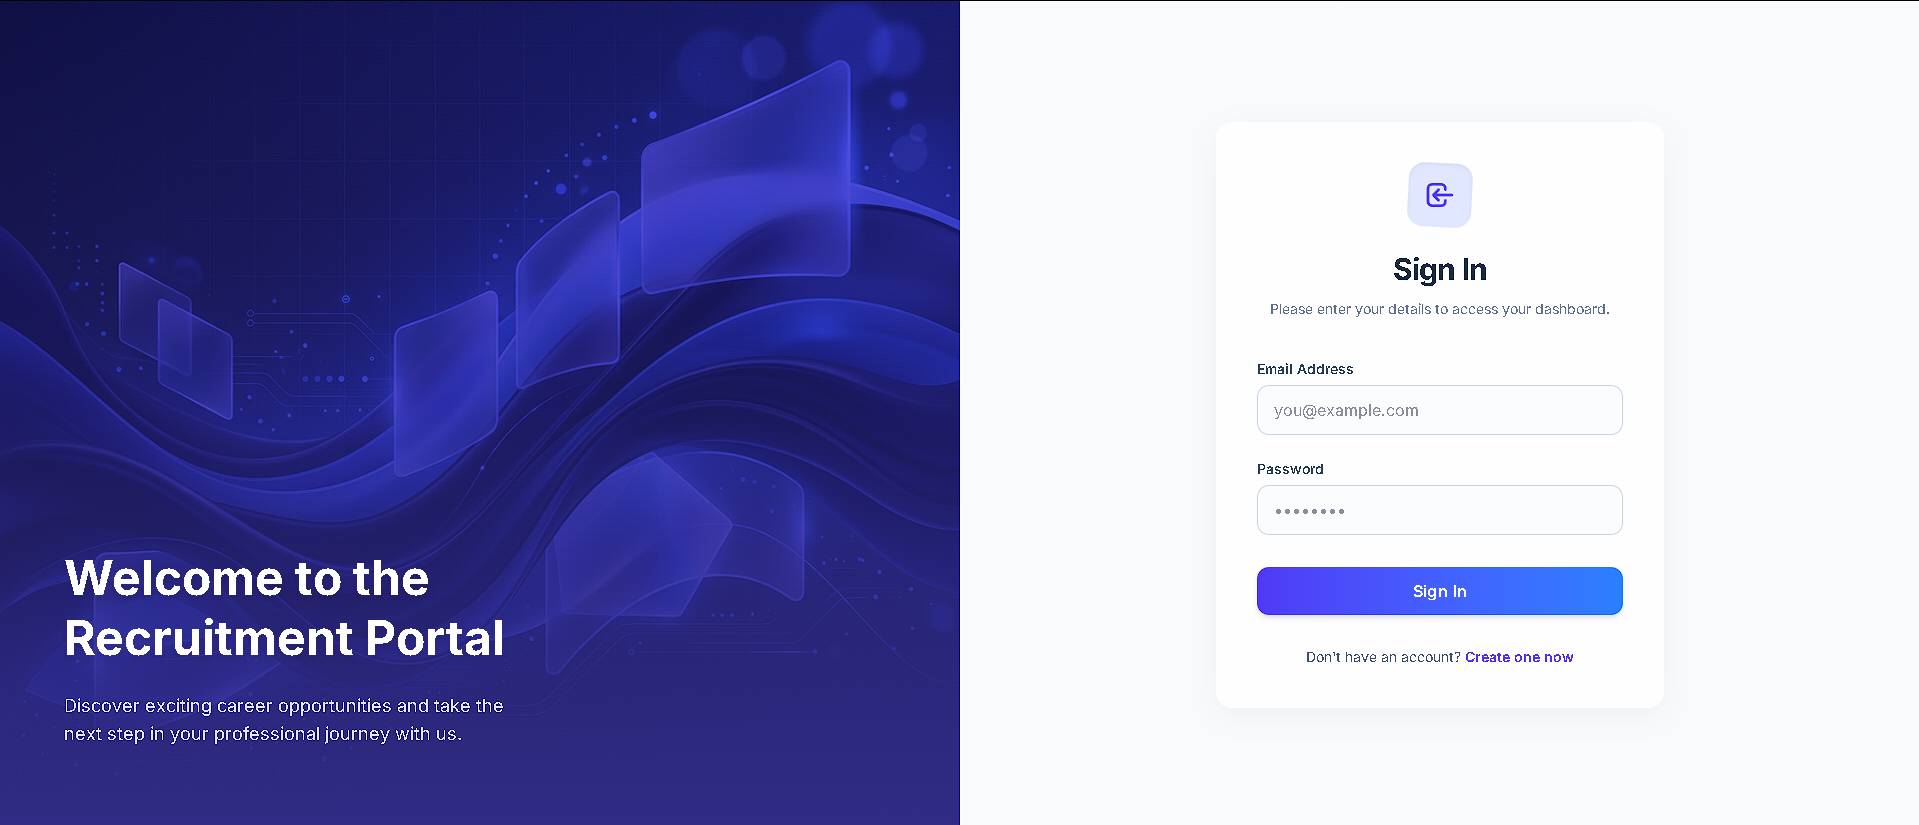
\includegraphics[width=\textwidth]{figures/student_login.png}}
    \caption{Student Login.}
  \end{minipage}\hfill
  \begin{minipage}{0.48\textwidth}
    \centering
    \fbox{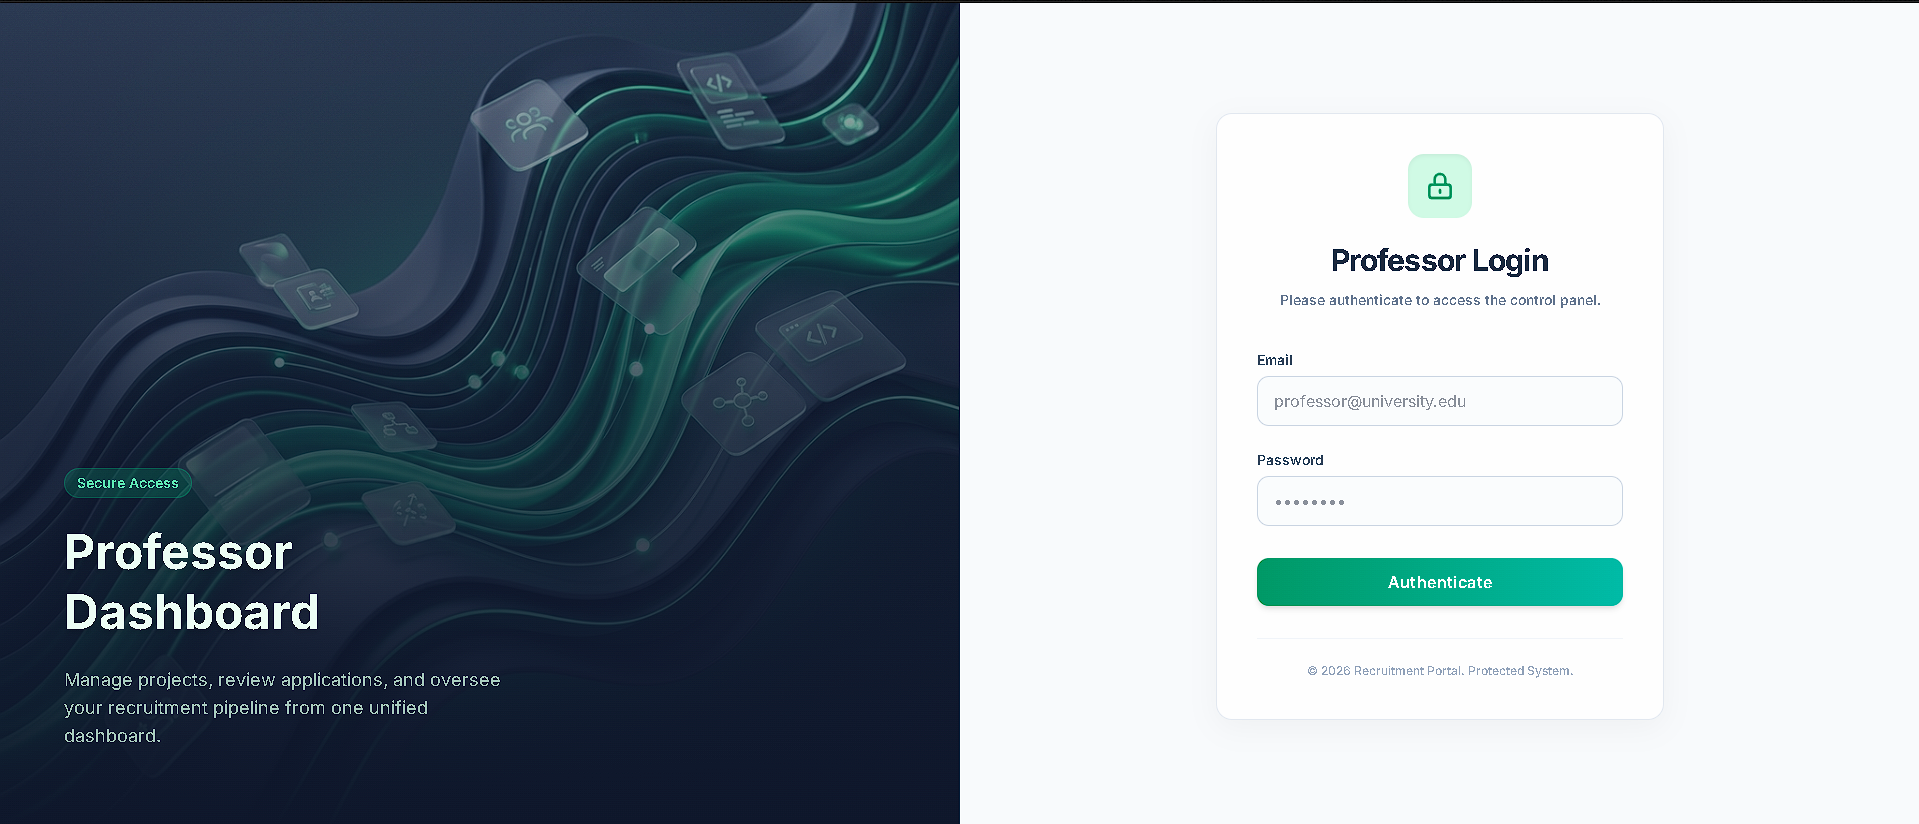
\includegraphics[width=\textwidth]{figures/professor_login.png}}
    \caption{Professor Login.}
  \end{minipage}
  
  \vspace{1ex}
  
  \begin{minipage}{0.48\textwidth}
    \centering
    \fbox{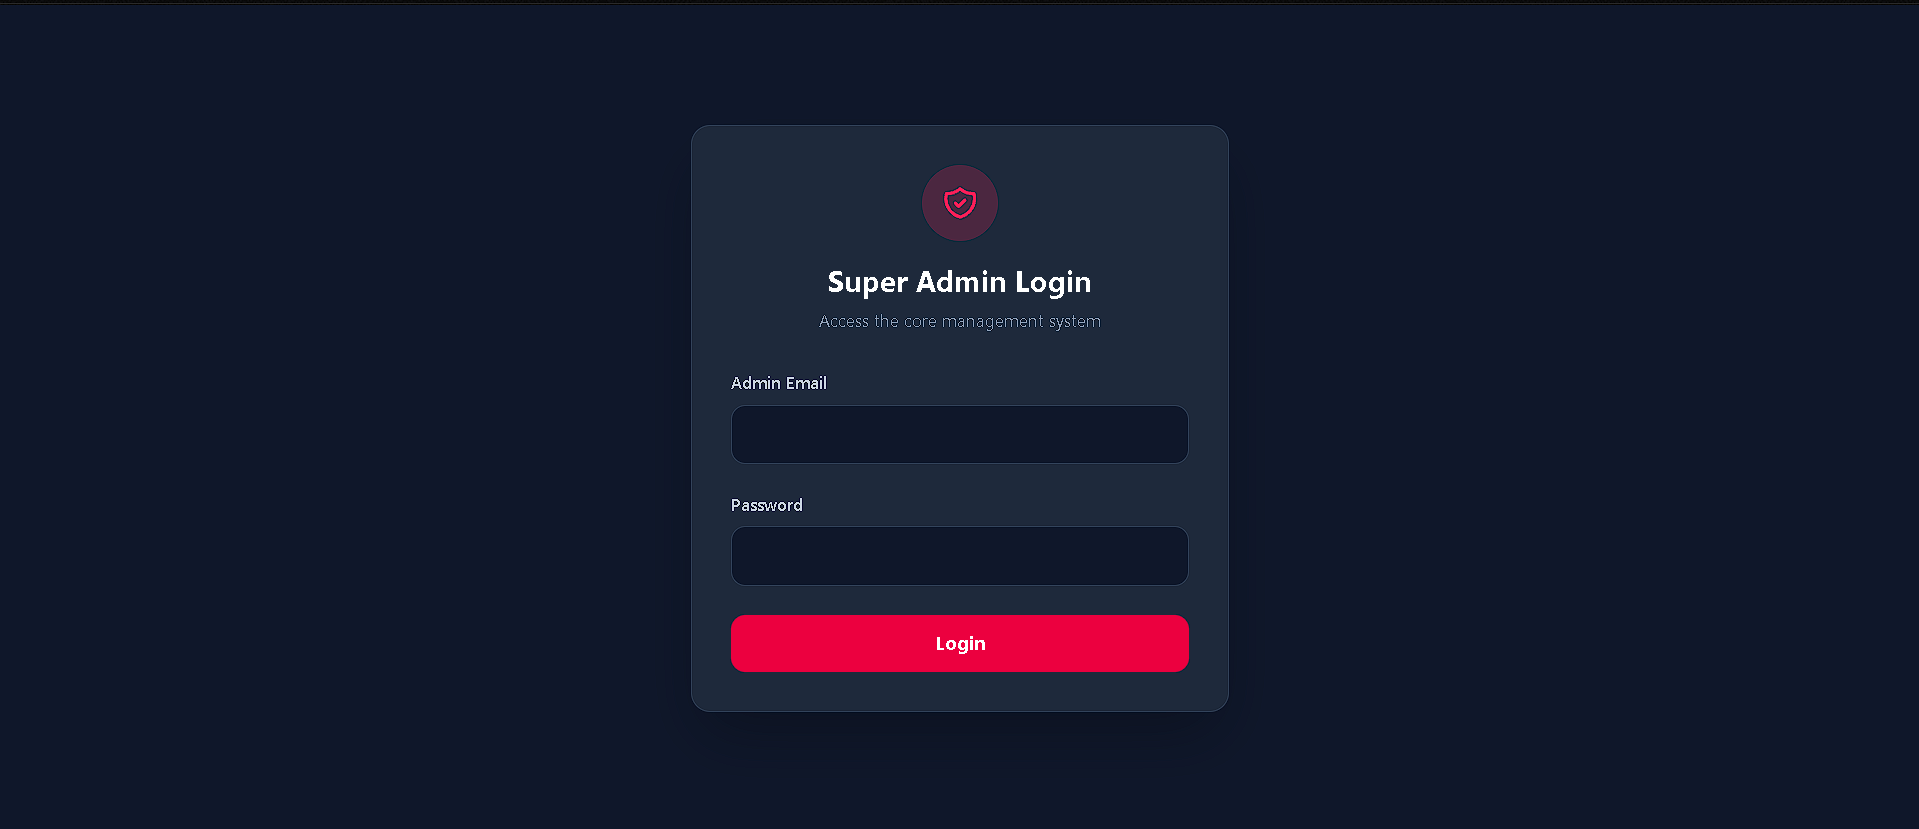
\includegraphics[width=\textwidth]{figures/admin_login.png}}
    \caption{Admin Login.}
  \end{minipage}
\end{figure}

\subsubsection{Professor Workflow}

Professors can create new project listings and manage applications received for their projects.

\begin{figure}[H]
  \centering
  \setlength{\fboxsep}{0pt}
  \setlength{\fboxrule}{0.2pt}
  \fbox{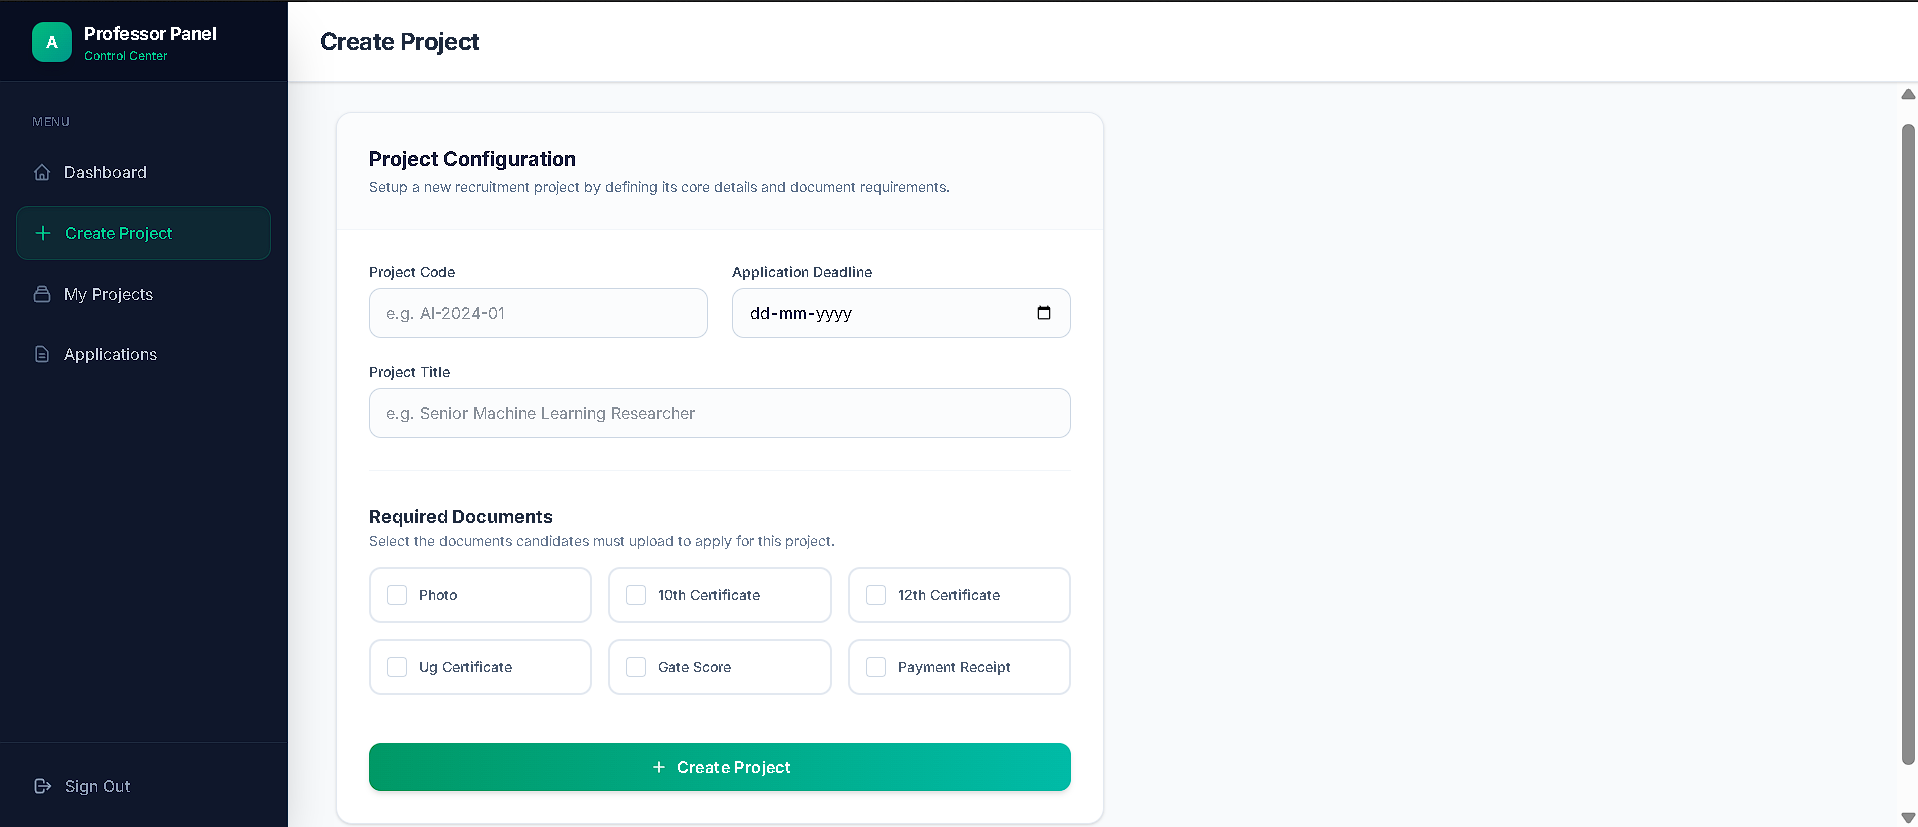
\includegraphics[width=0.85\textwidth]{figures/create_project.png}}
  \caption{Interface for creating a new project listing.}
  \label{fig:create_proj}
\end{figure}

\begin{figure}[H]
  \centering
  \setlength{\fboxsep}{0pt}
  \setlength{\fboxrule}{0.2pt}
  \fbox{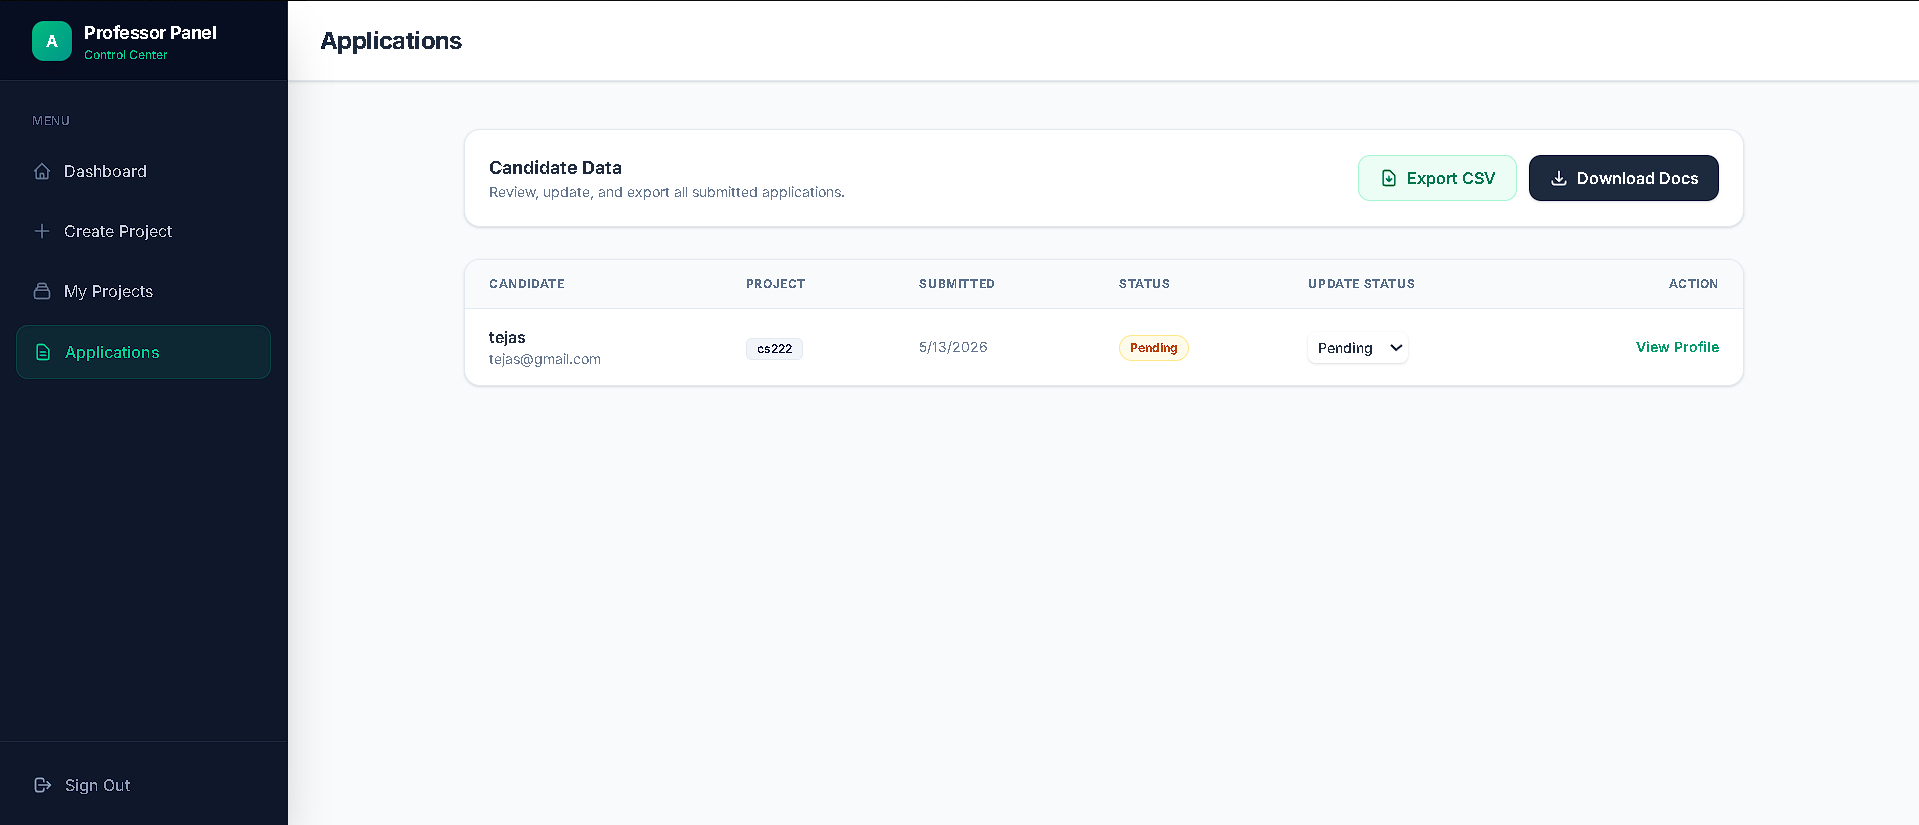
\includegraphics[width=0.85\textwidth]{figures/professor_studentapplications.png}}
  \caption{Professor's view of students who applied for a specific project.}
  \label{fig:prof_apps}
\end{figure}

\subsubsection{Administrative Management}

The Administrator has tools to moderate projects and view applications across the entire institution.

\begin{figure}[H]
  \centering
  \setlength{\fboxsep}{0pt}
  \setlength{\fboxrule}{0.2pt}
  \fbox{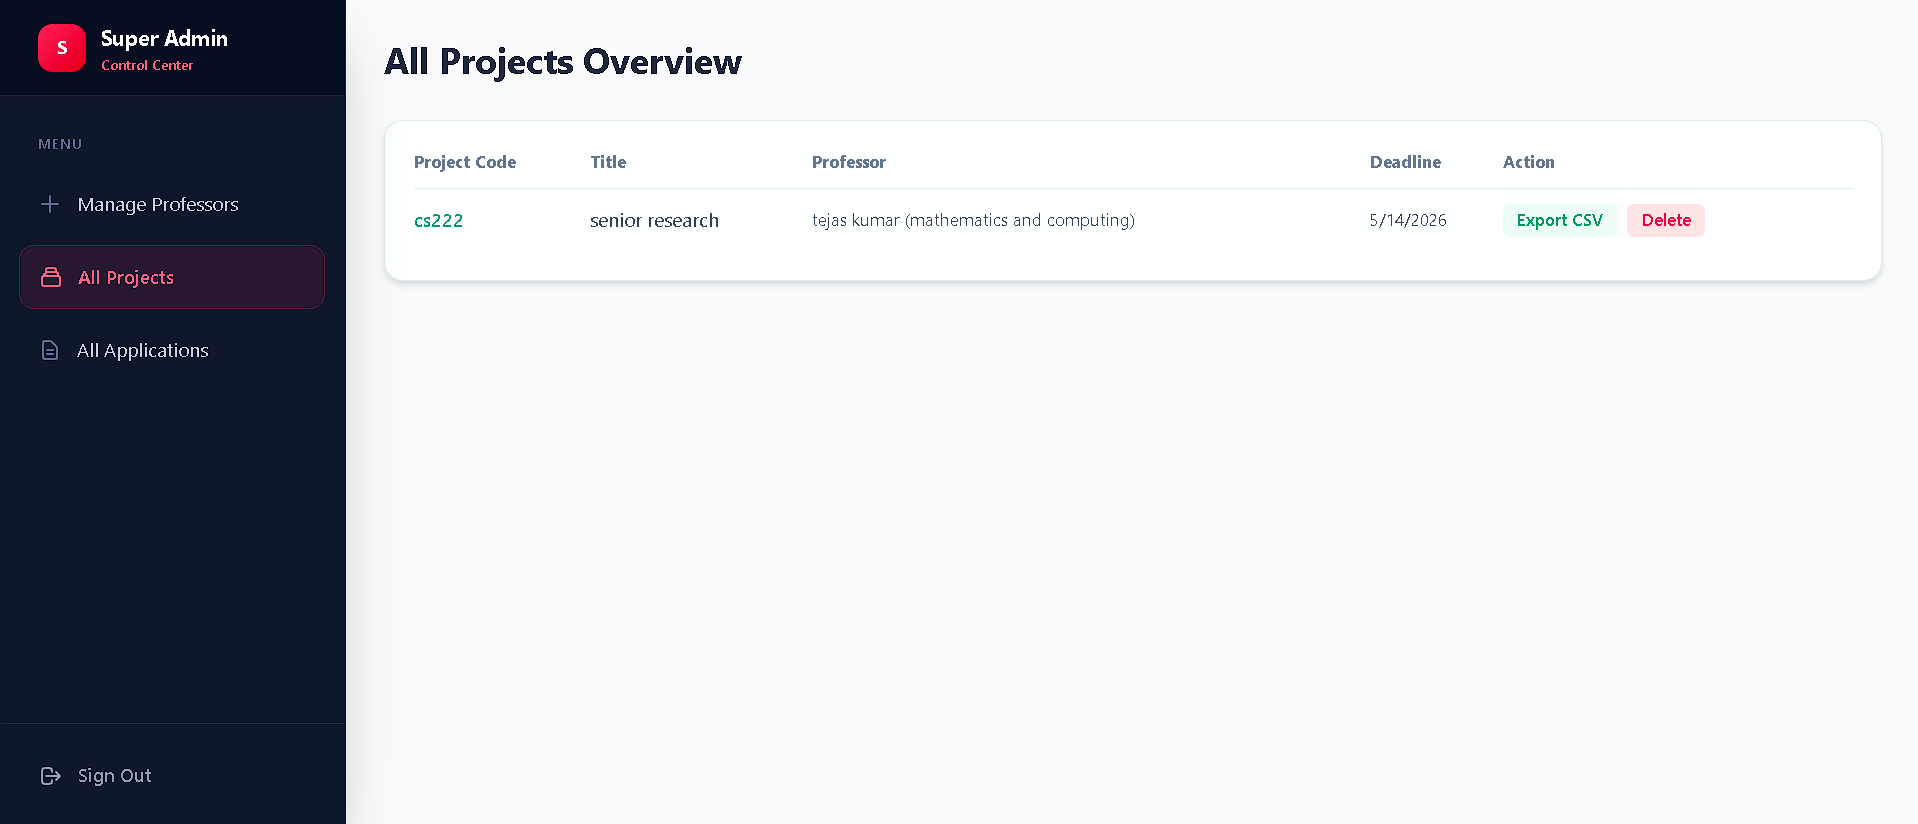
\includegraphics[width=0.85\textwidth]{figures/admin_allprojectoverview.png}}
  \caption{Admin overview of all projects currently listed on the portal.}
  \label{fig:admin_proj}
\end{figure}

\begin{figure}[H]
  \centering
  \setlength{\fboxsep}{0pt}
  \setlength{\fboxrule}{0.2pt}
  \fbox{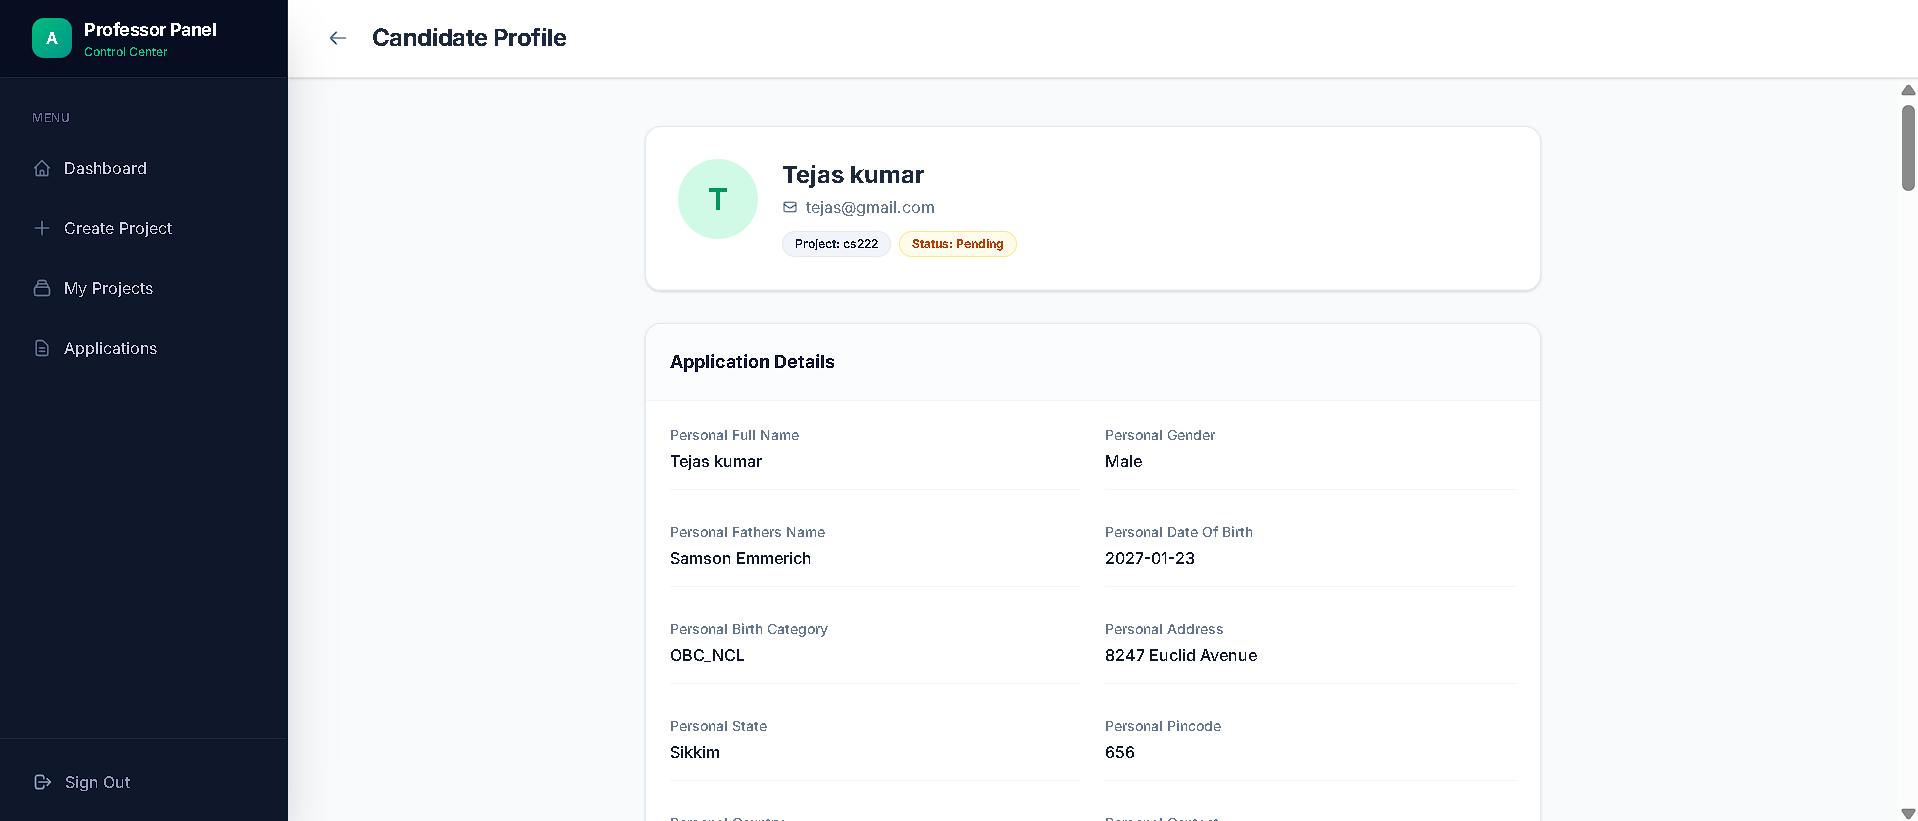
\includegraphics[width=0.85\textwidth]{figures/studentapplication_viewprofile.png}}
  \caption{Detailed view of an applicant's profile and submitted documents.}
  \label{fig:app_profile}
\end{figure}

\begin{figure}[H]
  \centering
  \setlength{\fboxsep}{0pt}
  \setlength{\fboxrule}{0.2pt}
  \fbox{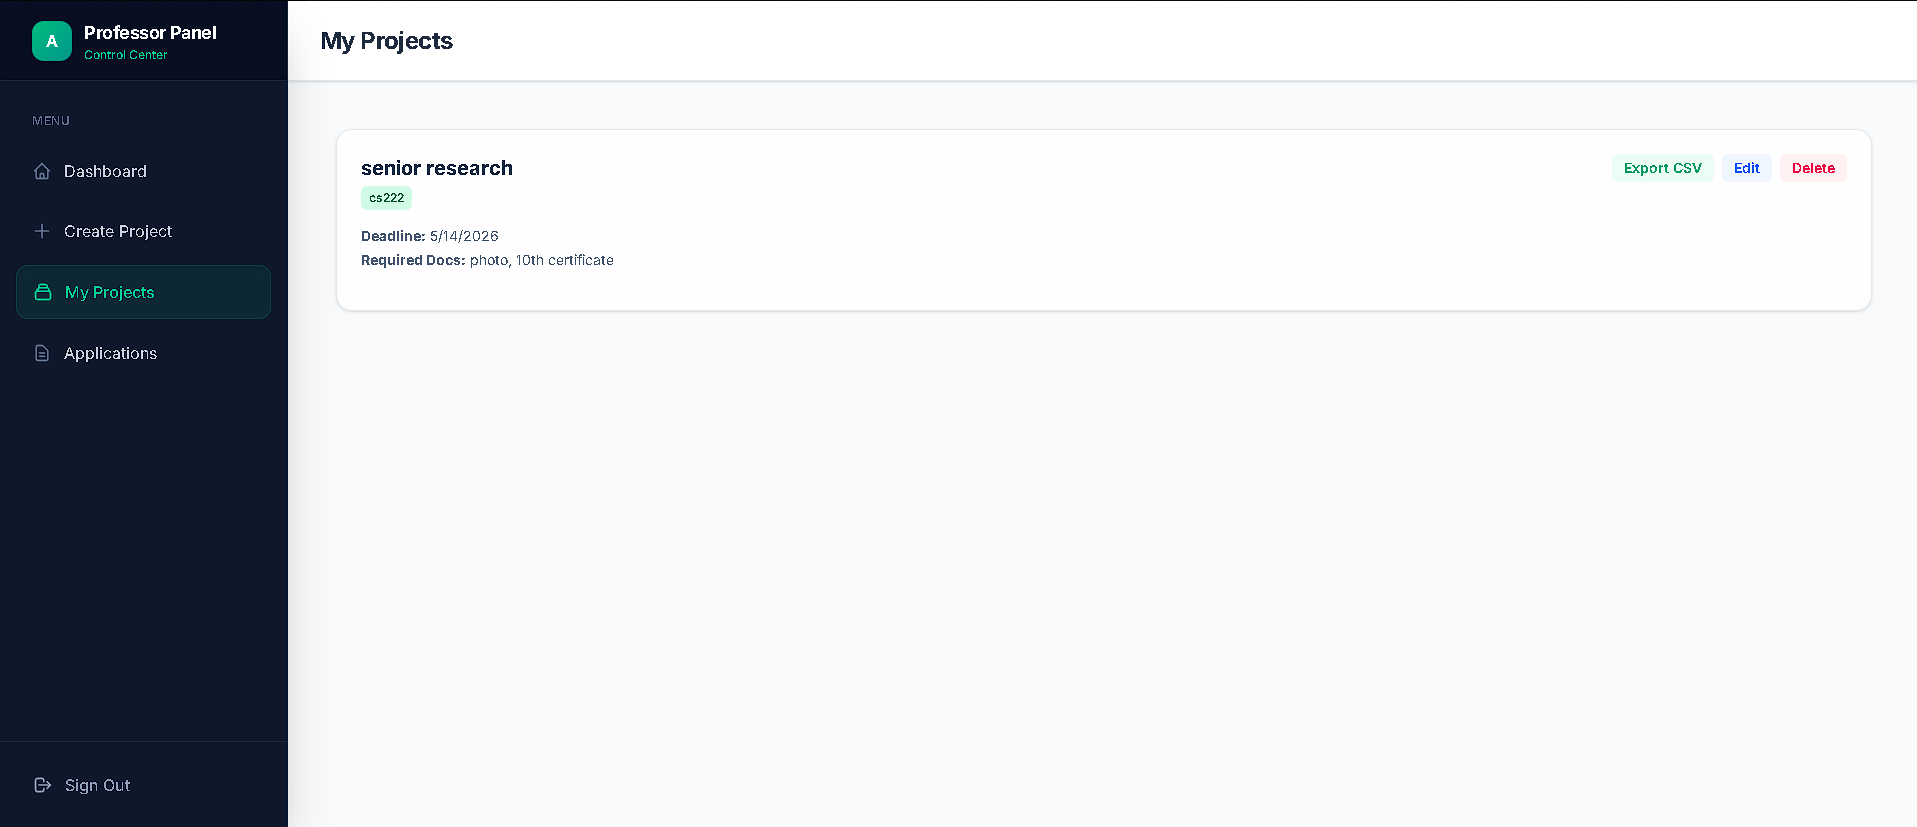
\includegraphics[width=0.85\textwidth]{figures/professor_myproject.png}}
  \caption{Professor's management view listing all projects created by them.}
  \label{fig:prof_projects}
\end{figure}

\begin{figure}[H]
  \centering
  \setlength{\fboxsep}{0pt}
  \setlength{\fboxrule}{0.2pt}
  \fbox{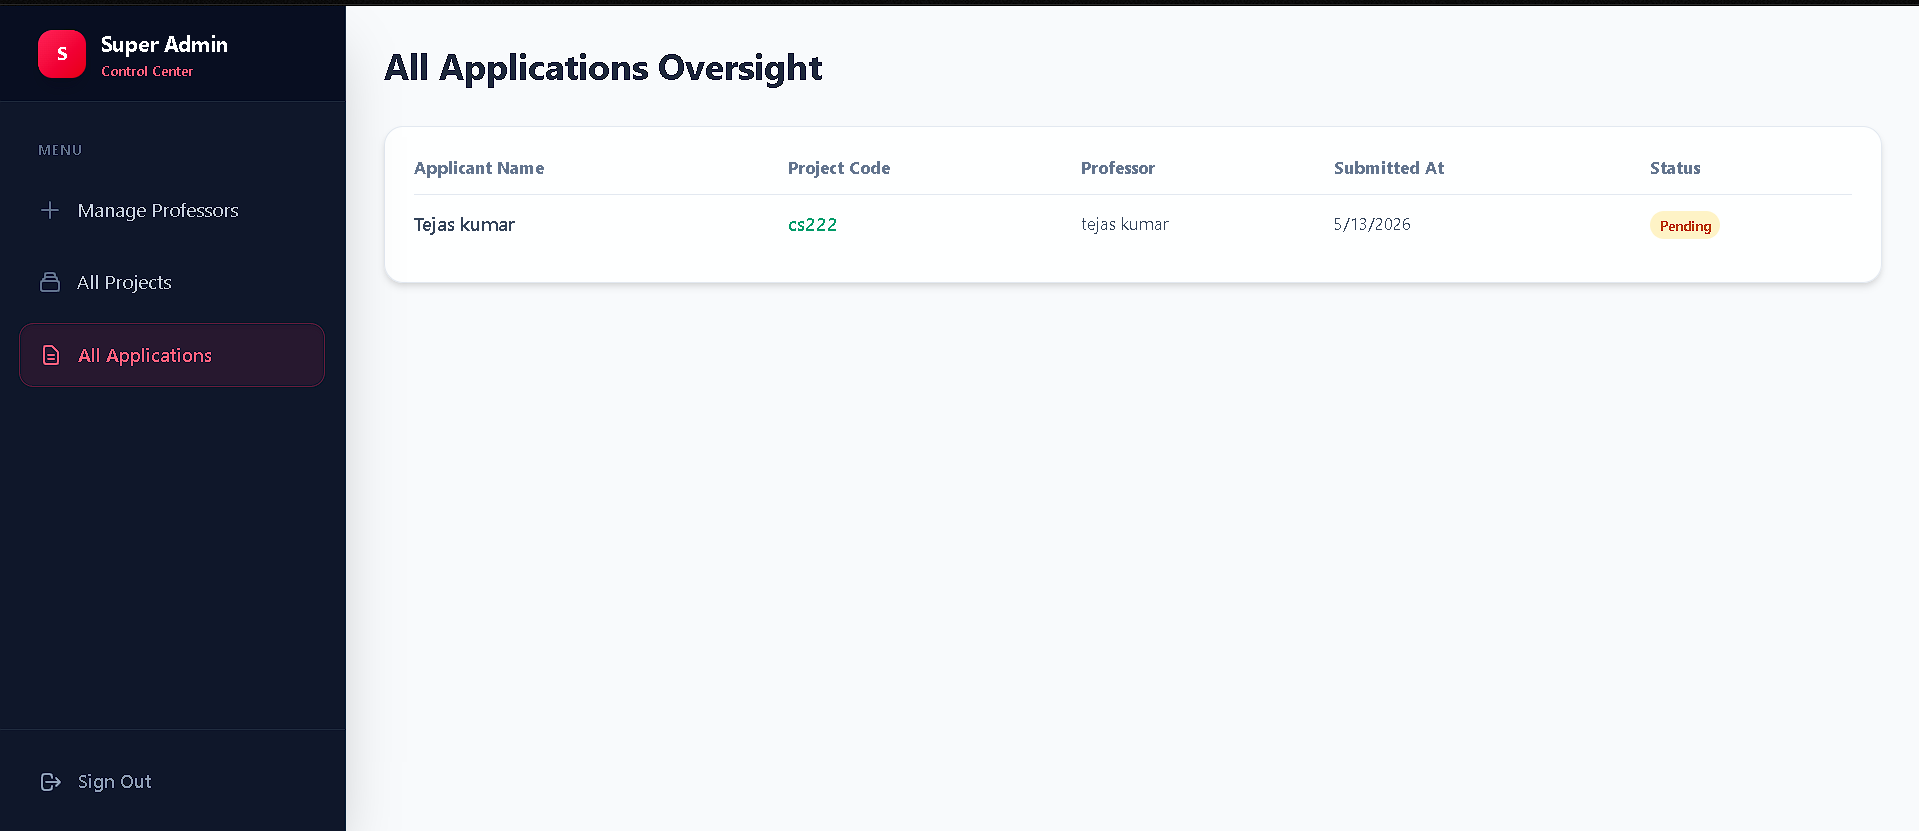
\includegraphics[width=0.85\textwidth]{figures/admin_allapplications.png}}
  \caption{Admin view showing all applications received across all institutional projects.}
  \label{fig:admin_apps}
\end{figure}

\section{Deployment and Containerization}

The system is containerized into three main services: `backend`, `frontend`, and `database`. Docker Compose manages the orchestration and networking between these services.

\begin{lstlisting}[language=bash, caption={Docker Compose service overview.}]
services:
  backend:
    build: ./backend
    volumes:
      - uploads_data:/app/uploads
  frontend:
    build: ./frontend
  db:
    image: mongo:latest
\end{lstlisting}

A named volume `uploads_data` is used to persist uploaded files outside the backend container's ephemeral storage.

\section{Security Implementation}

The system integrates several security hardening measures to protect sensitive applicant data. Table~\ref{tab:security} summarizes the key security features and the specific threats they mitigate.

\begin{table}[H]
  \centering
  \caption{Security features and threat mitigation in the Recruitment Portal.}
  \label{tab:security}
  \begin{tabularx}{\textwidth}{lX}
    \hline
    \textbf{Security Feature} & \textbf{Threat Mitigation} \\
    \hline
    Bcrypt Hashing (12 rounds) & Protects user passwords against brute-force and rainbow table attacks. \\
    JWT (Stateless Auth)       & Mitigates session fixation and CSRF risks by avoiding server-side session state. \\
    Express Validator          & Prevents NoSQL injection and XSS by sanitizing all incoming request bodies. \\
    Helmet.js Headers          & Enables CSP and HSTS to protect against cross-site scripting and protocol downgrades. \\
    Rate Limiting              & Protects the login and registration endpoints from automated dictionary attacks. \\
    \hline
  \end{tabularx}
\end{table}
